% Options for packages loaded elsewhere
\PassOptionsToPackage{unicode}{hyperref}
\PassOptionsToPackage{hyphens}{url}
%
\documentclass[
  ignorenonframetext,
  aspectratio=169]{beamer}
\usepackage{pgfpages}
\setbeamertemplate{caption}[numbered]
\setbeamertemplate{caption label separator}{: }
\setbeamercolor{caption name}{fg=normal text.fg}
\beamertemplatenavigationsymbolsempty
% Prevent slide breaks in the middle of a paragraph
\widowpenalties 1 10000
\raggedbottom
\setbeamertemplate{part page}{
  \centering
  \begin{beamercolorbox}[sep=16pt,center]{part title}
    \usebeamerfont{part title}\insertpart\par
  \end{beamercolorbox}
}
\setbeamertemplate{section page}{
  \centering
  \begin{beamercolorbox}[sep=12pt,center]{part title}
    \usebeamerfont{section title}\insertsection\par
  \end{beamercolorbox}
}
\setbeamertemplate{subsection page}{
  \centering
  \begin{beamercolorbox}[sep=8pt,center]{part title}
    \usebeamerfont{subsection title}\insertsubsection\par
  \end{beamercolorbox}
}
\AtBeginPart{
  \frame{\partpage}
}
\AtBeginSection{
  \ifbibliography
  \else
    \frame{\sectionpage}
  \fi
}
\AtBeginSubsection{
  \frame{\subsectionpage}
}
\usepackage{lmodern}
\usepackage{amssymb,amsmath}
\usepackage{ifxetex,ifluatex}
\ifnum 0\ifxetex 1\fi\ifluatex 1\fi=0 % if pdftex
  \usepackage[T1]{fontenc}
  \usepackage[utf8]{inputenc}
  \usepackage{textcomp} % provide euro and other symbols
\else % if luatex or xetex
  \usepackage{unicode-math}
  \defaultfontfeatures{Scale=MatchLowercase}
  \defaultfontfeatures[\rmfamily]{Ligatures=TeX,Scale=1}
\fi
\usetheme[]{Frankfurt}
\usefonttheme{structurebold}
% Use upquote if available, for straight quotes in verbatim environments
\IfFileExists{upquote.sty}{\usepackage{upquote}}{}
\IfFileExists{microtype.sty}{% use microtype if available
  \usepackage[]{microtype}
  \UseMicrotypeSet[protrusion]{basicmath} % disable protrusion for tt fonts
}{}
\makeatletter
\@ifundefined{KOMAClassName}{% if non-KOMA class
  \IfFileExists{parskip.sty}{%
    \usepackage{parskip}
  }{% else
    \setlength{\parindent}{0pt}
    \setlength{\parskip}{6pt plus 2pt minus 1pt}}
}{% if KOMA class
  \KOMAoptions{parskip=half}}
\makeatother
\usepackage{xcolor}
\IfFileExists{xurl.sty}{\usepackage{xurl}}{} % add URL line breaks if available
\IfFileExists{bookmark.sty}{\usepackage{bookmark}}{\usepackage{hyperref}}
\hypersetup{
  pdftitle={Generación de informes reproducibles con RMarkdown},
  pdfauthor={Mg. Jesús Eduardo Gamboa Unsihuay},
  hidelinks,
  pdfcreator={LaTeX via pandoc}}
\urlstyle{same} % disable monospaced font for URLs
\newif\ifbibliography
\usepackage{color}
\usepackage{fancyvrb}
\newcommand{\VerbBar}{|}
\newcommand{\VERB}{\Verb[commandchars=\\\{\}]}
\DefineVerbatimEnvironment{Highlighting}{Verbatim}{commandchars=\\\{\}}
% Add ',fontsize=\small' for more characters per line
\usepackage{framed}
\definecolor{shadecolor}{RGB}{248,248,248}
\newenvironment{Shaded}{\begin{snugshade}}{\end{snugshade}}
\newcommand{\AlertTok}[1]{\textcolor[rgb]{0.94,0.16,0.16}{#1}}
\newcommand{\AnnotationTok}[1]{\textcolor[rgb]{0.56,0.35,0.01}{\textbf{\textit{#1}}}}
\newcommand{\AttributeTok}[1]{\textcolor[rgb]{0.77,0.63,0.00}{#1}}
\newcommand{\BaseNTok}[1]{\textcolor[rgb]{0.00,0.00,0.81}{#1}}
\newcommand{\BuiltInTok}[1]{#1}
\newcommand{\CharTok}[1]{\textcolor[rgb]{0.31,0.60,0.02}{#1}}
\newcommand{\CommentTok}[1]{\textcolor[rgb]{0.56,0.35,0.01}{\textit{#1}}}
\newcommand{\CommentVarTok}[1]{\textcolor[rgb]{0.56,0.35,0.01}{\textbf{\textit{#1}}}}
\newcommand{\ConstantTok}[1]{\textcolor[rgb]{0.00,0.00,0.00}{#1}}
\newcommand{\ControlFlowTok}[1]{\textcolor[rgb]{0.13,0.29,0.53}{\textbf{#1}}}
\newcommand{\DataTypeTok}[1]{\textcolor[rgb]{0.13,0.29,0.53}{#1}}
\newcommand{\DecValTok}[1]{\textcolor[rgb]{0.00,0.00,0.81}{#1}}
\newcommand{\DocumentationTok}[1]{\textcolor[rgb]{0.56,0.35,0.01}{\textbf{\textit{#1}}}}
\newcommand{\ErrorTok}[1]{\textcolor[rgb]{0.64,0.00,0.00}{\textbf{#1}}}
\newcommand{\ExtensionTok}[1]{#1}
\newcommand{\FloatTok}[1]{\textcolor[rgb]{0.00,0.00,0.81}{#1}}
\newcommand{\FunctionTok}[1]{\textcolor[rgb]{0.00,0.00,0.00}{#1}}
\newcommand{\ImportTok}[1]{#1}
\newcommand{\InformationTok}[1]{\textcolor[rgb]{0.56,0.35,0.01}{\textbf{\textit{#1}}}}
\newcommand{\KeywordTok}[1]{\textcolor[rgb]{0.13,0.29,0.53}{\textbf{#1}}}
\newcommand{\NormalTok}[1]{#1}
\newcommand{\OperatorTok}[1]{\textcolor[rgb]{0.81,0.36,0.00}{\textbf{#1}}}
\newcommand{\OtherTok}[1]{\textcolor[rgb]{0.56,0.35,0.01}{#1}}
\newcommand{\PreprocessorTok}[1]{\textcolor[rgb]{0.56,0.35,0.01}{\textit{#1}}}
\newcommand{\RegionMarkerTok}[1]{#1}
\newcommand{\SpecialCharTok}[1]{\textcolor[rgb]{0.00,0.00,0.00}{#1}}
\newcommand{\SpecialStringTok}[1]{\textcolor[rgb]{0.31,0.60,0.02}{#1}}
\newcommand{\StringTok}[1]{\textcolor[rgb]{0.31,0.60,0.02}{#1}}
\newcommand{\VariableTok}[1]{\textcolor[rgb]{0.00,0.00,0.00}{#1}}
\newcommand{\VerbatimStringTok}[1]{\textcolor[rgb]{0.31,0.60,0.02}{#1}}
\newcommand{\WarningTok}[1]{\textcolor[rgb]{0.56,0.35,0.01}{\textbf{\textit{#1}}}}
\setlength{\emergencystretch}{3em} % prevent overfull lines
\providecommand{\tightlist}{%
  \setlength{\itemsep}{0pt}\setlength{\parskip}{0pt}}
\setcounter{secnumdepth}{-\maxdimen} % remove section numbering
\definecolor{greeen}{RGB}{66,144,94}
\setbeamercolor{palette primary}{use=structure,fg=white,bg=greeen}

\title{Generación de informes reproducibles con RMarkdown}
\subtitle{Día del estadístico peruano}
\author{Mg. Jesús Eduardo Gamboa Unsihuay}
\date{05/12/2020}

\begin{document}
\frame{\titlepage}

\begin{frame}
  \tableofcontents[hideallsubsections]
\end{frame}
\hypertarget{introducciuxf3n}{%
\section{Introducción}\label{introducciuxf3n}}

\begin{frame}{Introducción}

\begin{figure}

\includegraphics[width=0.8\textwidth]{reproducible.jpg}
\end{figure}

\begin{center}
https://www.youtube.com/watch?v=s3JldKoA0zw
\end{center}

\end{frame}

\begin{frame}

\begin{figure}
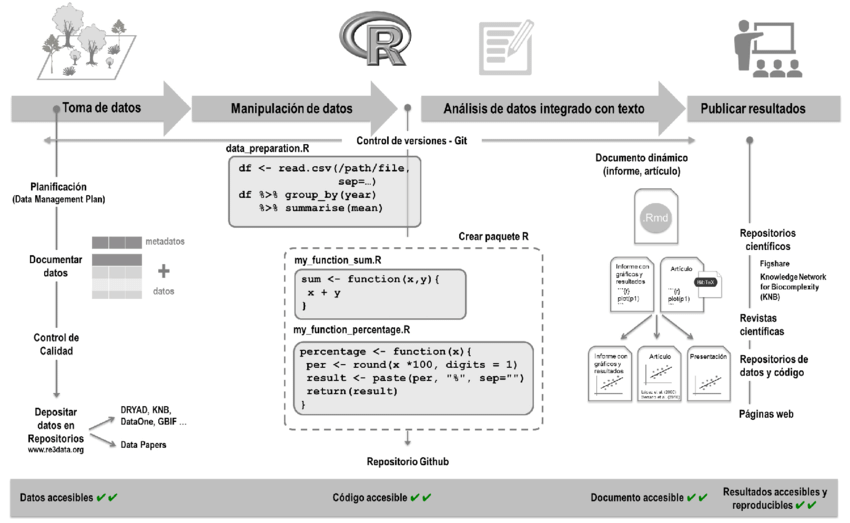
\includegraphics[width=0.8\textwidth]{flujo.png}
\end{figure}

\end{frame}

\hypertarget{proyectos-en-rstudio}{%
\section{Proyectos en RStudio}\label{proyectos-en-rstudio}}

\begin{frame}{Proyectos en RStudio}

Reflexionemos acerca de nuestro modo de trabajo en RStudio:

\begin{enumerate}
\item
  ¿Tus datos son `vecinos' de tus scripts?
\item
  ¿Cómo lees conjuntos de datos?
\item
  ¿Cargas el espacio de trabajo al iniciar sesión? ¿lo guardas al
  finalizar?
\end{enumerate}

\end{frame}

\begin{frame}

\begin{block}{Los datos como `vecinos' de los scripts}

\begin{itemize}
\item
  Evitar casos como este:

  \begin{center}
  \texttt{read.csv("C:/Documentos/Curso Regresion/Trabajo 1/datos.csv")}
  \texttt{read.delim("clipboard")}
  \end{center}
\item
  Datos vecinos de los scripts \(\rightarrow\) facilitará la lectura.
\item
  No será necesario indicar la ruta:

  \begin{center}
  \texttt{read.csv("datos.csv")}
  \end{center}
\end{itemize}

\end{block}

\end{frame}

\begin{frame}[fragile]

\begin{block}{Lectura de datos}

Ejemplo:

\begin{Shaded}
\begin{Highlighting}[]
\NormalTok{datos <-}\StringTok{ }\KeywordTok{read.csv2}\NormalTok{(}\StringTok{"datos.csv"}\NormalTok{, }\DataTypeTok{dec =} \StringTok{"."}\NormalTok{)}
\NormalTok{datos}
\end{Highlighting}
\end{Shaded}

\begin{verbatim}
##    X     Y
## 1  2 12.06
## 2  6 32.83
## 3  1  8.28
## 4  6 32.39
## 5  4 21.59
## 6  3 17.61
## 7 10 53.10
## 8  7 35.74
\end{verbatim}

\end{block}

\end{frame}

\begin{frame}[fragile]

\begin{block}{Manipulación de datos}

\begin{itemize}
\item
  Use R para limpiar, transformar y manipular conjuntos de datos
\item
  Funciones de manipulación en el paquete \textbf{dplyr}: filter,
  select, mutate, etc.
\end{itemize}

\begin{Shaded}
\begin{Highlighting}[]
\KeywordTok{library}\NormalTok{(dplyr)}
\NormalTok{datos2 <-}\StringTok{ }\NormalTok{datos }\OperatorTok\StringTok{ }
\StringTok{  }\KeywordTok{mutate}\NormalTok{(}\DataTypeTok{Z =}\NormalTok{ Y }\OperatorTok{-}\StringTok{ }\NormalTok{X)}
\end{Highlighting}
\end{Shaded}

\end{block}

\end{frame}

\begin{frame}[fragile]

\begin{block}{No cargar ni guardar espacio de trabajo}

\begin{itemize}
\item
  Guardar códigos en vez de almacenar el espacio de trabajo
\item
  De ser necesario almacenar un objeto, hacerlo en formato RDS en vez de
  Rda o RData
\item
  Ejemplo:
\end{itemize}

\begin{Shaded}
\begin{Highlighting}[]
\NormalTok{modelo <-}\StringTok{ }\KeywordTok{lm}\NormalTok{(Y }\OperatorTok{~}\StringTok{ }\NormalTok{X, }\DataTypeTok{data =}\NormalTok{ datos)}
\KeywordTok{saveRDS}\NormalTok{(modelo, }\StringTok{"modeloRL.RDS"}\NormalTok{)}
\end{Highlighting}
\end{Shaded}

\end{block}

\end{frame}

\begin{frame}[fragile]{Exportando objetos}
\protect\hypertarget{exportando-objetos}{}

\begin{Shaded}
\begin{Highlighting}[]
\KeywordTok{write.csv}\NormalTok{(datos2,}\StringTok{"datos2.csv"}\NormalTok{)}
\KeywordTok{library}\NormalTok{(ggplot2)}
\NormalTok{imagen =}\StringTok{ }\KeywordTok{ggplot}\NormalTok{(datos, }\KeywordTok{aes}\NormalTok{(X,Y)) }\OperatorTok{+}
\StringTok{  }\KeywordTok{geom_point}\NormalTok{() }\OperatorTok{+}\StringTok{ }\KeywordTok{theme_minimal}\NormalTok{()}
\KeywordTok{ggsave}\NormalTok{(}\StringTok{"imagen.png"}\NormalTok{,imagen)}
\end{Highlighting}
\end{Shaded}

\end{frame}

\begin{frame}{Algunos puntos adicionales}
\protect\hypertarget{algunos-puntos-adicionales}{}

\begin{itemize}
\item
  No colocar \textbf{install.packages(``\ldots{}'')} en código
  reproducible.
\item
  Los proyectos son el punto de partida para la creación de paquetes
\end{itemize}

\end{frame}

\hypertarget{trabajando-con-rmarkdown}{%
\section{Trabajando con RMarkdown}\label{trabajando-con-rmarkdown}}

\begin{frame}{Trabajando con RMarkdown}

\begin{center}

\begin{figure}

\includegraphics[width=0.25\textwidth]{rmarkdown.png}
\end{figure}

Texto + código + resultados

\textbf{https://rstudio.com/wp-content/uploads/2015/02/rmarkdown-cheatsheet.pdf}
\end{center}

\end{frame}

\begin{frame}

\begin{figure}
\includegraphics[width=0.9\textwidth]{rmarkdown_components.png}
\end{figure}

\end{frame}

\begin{frame}

\begin{itemize}
\item
  Documentos \(\rightarrow\) HTML, PDF, Word
\item
  Presentaciones \(\rightarrow\) HTML, PDF, Power Point
\item
  Dashboard estático (flexdashboard)
\item
  Dashborad interactivo (shiny)
\item
  Tutorial (learnr)
\item
  Blog (distill)
\item
  Libro (bookdown)
\item
  Publicacion en GitHub
\item
  Publicación en RPubs
\end{itemize}

\end{frame}

\begin{frame}

\textbf{Ejemplo Flexdashboard + RPubs}

\begin{figure}
\includegraphics[width=0.9\textwidth]{rpubs.jpg}
\end{figure}

\begin{center}
\textbf{https://rpubs.com/jesuseduardog/covid19peru}
\end{center}

\end{frame}

\begin{frame}

Esta presentación está alojada en

\begin{center}
\textbf{https://github.com/jeguns/reproducibilidad}
\end{center}

Contacto:
\href{mailto:jgamboa@lamolina.edu.pe}{\nolinkurl{jgamboa@lamolina.edu.pe}}

\end{frame}

\end{document}
